\documentclass{article}
\usepackage{amsmath}
\usepackage{tikz}
\usetikzlibrary{arrows.meta}

\begin{document}

\textit{Left}: Representation of the pairwise Transfer Entropy \( T_{p} \) and of the values obtained maximizing and minimizing \( T_{\alpha} \), called \( T_{M} \) and \( T_{m} \) respectively. Redundant influences are depicted by red arrows, and synergistic influences by blue arrows.

\textit{Right}: Pairwise, synergistic, and redundant conditioning path are represented on a simple model with four nodes, with simulated couplings indicated by the dashed gray arrows.

\begin{figure}[h]
    \centering
    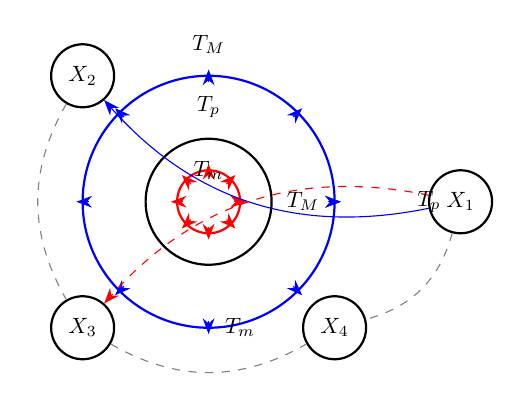
\begin{tikzpicture}[scale=0.8, every node/.style={transform shape}]
        
        % Left Diagram
        \draw[thick, blue] (0,0) circle (2);
        \draw[thick, black] (0,0) circle (1);
        \draw[thick, red] (0,0) circle (0.5);
        
        \foreach \angle in {0,45,...,360} {
            \draw[blue, -{Stealth[length=2mm]}] (\angle:1.9) -- (\angle:2.1);
            \draw[red, -{Stealth[length=2mm]}, dashed] (\angle:0.4) -- (\angle:0.6);
        }
        
        \node at (0, 2.5) {$T_{M}$};
        \node at (0, 1.5) {$T_{p}$};
        \node at (0, 0.5) {$T_{m}$};
        
        % Right Diagram
        \node[circle, draw, thick, minimum size=1cm] (X1) at (4,0) {$X_1$};
        \node[circle, draw, thick, minimum size=1cm] (X2) at (-2,2) {$X_2$};
        \node[circle, draw, thick, minimum size=1cm] (X3) at (-2,-2) {$X_3$};
        \node[circle, draw, thick, minimum size=1cm] (X4) at (2,-2) {$X_4$};
        
        \draw[blue, -{Stealth[length=2mm]}] (X1) to[bend left=30] (X2);
        \draw[red, -{Stealth[length=2mm]}, dashed] (X1) to[bend right=30] (X3);
        \draw[gray, dashed] (X1) to[bend left=30] (X4);
        \draw[gray, dashed] (X2) to[bend right=30] (X3);
        \draw[gray, dashed] (X3) to[bend right=30] (X4);
        
        \node at (3.5, 0) {$T_{p}$};
        \node at (1.5, 0) {$T_{M}$};
        \node at (0.5, -2) {$T_{m}$};
        
    \end{tikzpicture}
\end{figure}

\end{document}